\section{РЕАЛИЗАЦИЯ И ИСПОЛЬЗОВАНИЕ}
\label{sec:manual}

После изучения иструментов разработки и построенной архетектуре осталось реализовать приложение.
В данной работе реализованы десктопное приложение и модернизирована клиентская часть приложения. Десктопное приложение это основное приложение через которое осуществляется сканирование. Клиентская часть это скрипты вызова десктопного приложения, а так же источник ключевых данных для прикрепления документо. Создание основного приложения включает следующие
задачи:
\begin{itemize}
  \item создание внутренних функций для получения отсканированных изображений;
  \item создание внутренних функций для взаимодействи с сервером системы документооборота;
  \item создание SignalR соединения с клиентом;
  \item создание внутренних функций для изменения отсканированнх изображений;
  \item создание функционала для обработки изображений разного формата.
\end{itemize}

В первом пункте для работы со сканером используется библиотека VintaSoft TWAIN .NET. Второй пункт подразумевает прикрепление документов (отправка на сервер СЭД). Данная задача использует технологию WCF. Третий пункт создает SignalR сервер на стороне десктопного приложения. Клиентская часть устанавливает соединений, и когда прикрепление будет завершено, десктопное приложение отправит оповещение для обновления странички в браузере, где будет отображен только что прикрепленный файл.

Также стоит упомянуть про расширение клиентской части СЭД. Расширение клиентской части включало следующие задач   и:
\begin{itemize}
	\item создание функционала для сбора сведений о документе, к которому будет прикреплен отсканированный документ, и дальнейшая их передача в десктопное приложение;
	\item реализация взаимодействия с пользователем;
	\item запуск десктопного приложения посредством CustomURI;
	\item работа с SignalR.
\end{itemize}

\subsection{Руководство пользователя}

Рассмотри функционал и возможности приложения.

\subsubsection{Главное окно}

Если приложение запустить через ярлык, либо если сессия была отвязана главное окно приложения будет выглядеть следующим образом (рисунок 7.1). В данном случае пользователь может сканированть документы, редактировать, удалять лишние страницы, изменять настройки, сделать несколько заходов сканирования. Но прикрепить документы можно будет только с действующей сессией.

\begin{figure}[h!]
\centering
	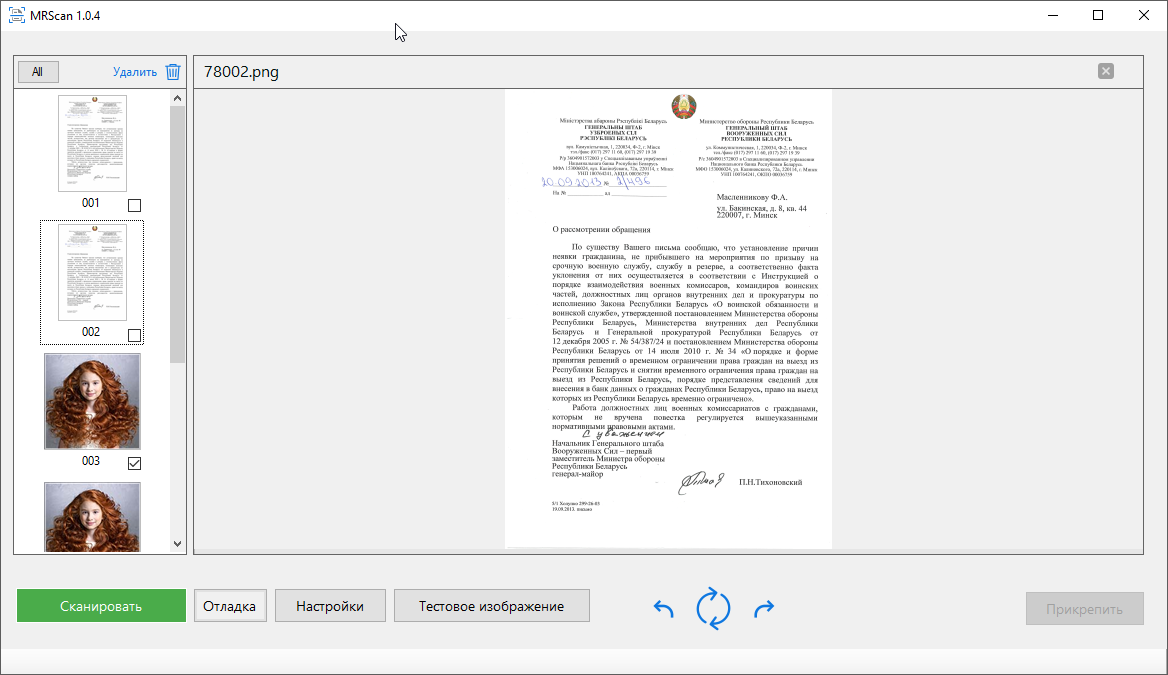
\includegraphics[scale=0.4]{main.png}
	\caption{Главное окно}
	\clearpage
\end{figure}

Для добавления сессии нужно перейти в клиентскую часть СЭД, выбрать документ к которому планируется прикрепить отсканированные файлы, перейти в окно работы с файлами и на панели с кнопками, нажать на кнопку «Сканировать» (рисунок 7.2).

\begin{figure}[h!]
\centering
	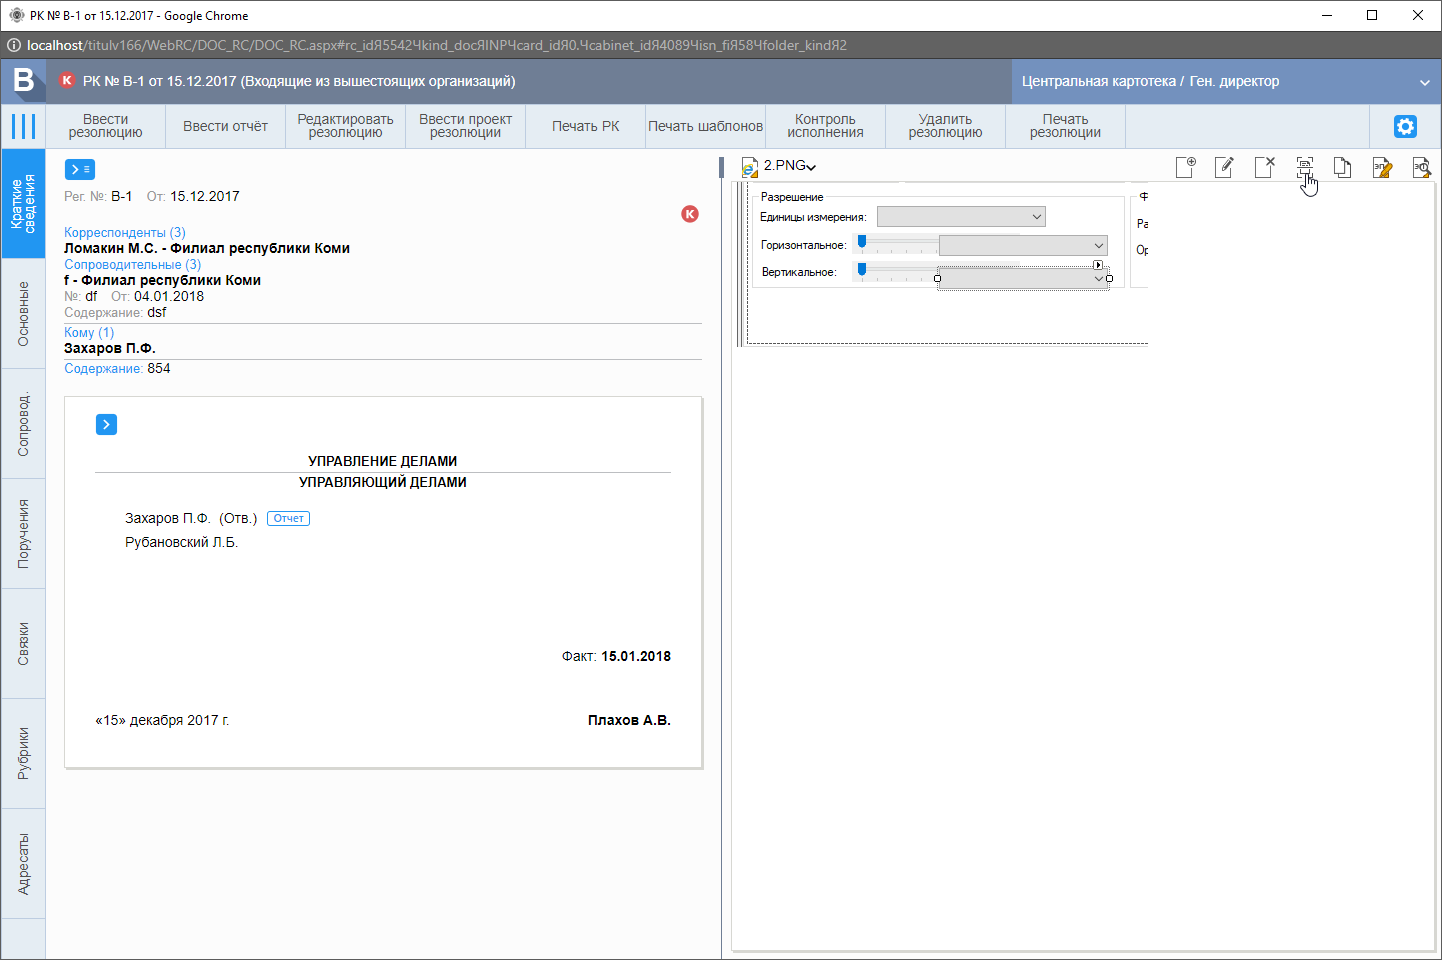
\includegraphics[scale=0.32]{titul.png}
	\caption{Веб версия СЭД}
	\clearpage
\end{figure}

После нажатия на кнопку «Сканировать», откроется всплывающее окно, где нужно будет подтвердить запуск десктопного приложения «MRScan». В разных браузерах окно может выглядеть по-разному. Скриншот из браузера Google Chrome (рисунок 7.3).

\begin{figure}[h!]
\centering
	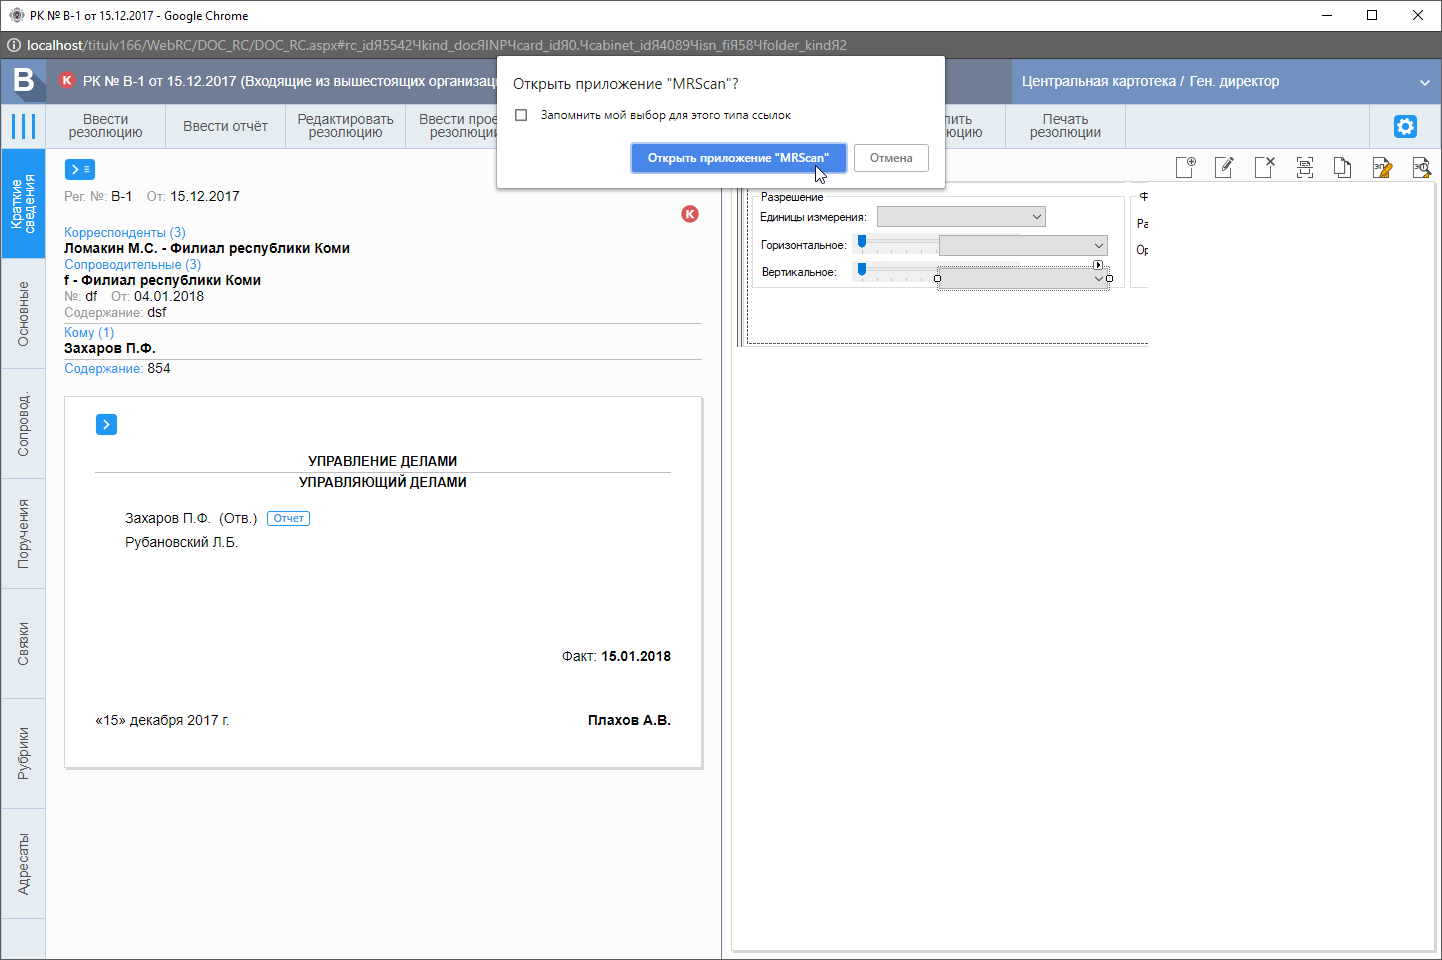
\includegraphics[scale=0.32]{titulCustom.png}
	\caption{Подтверждение запуска MRScan}
	\clearpage
\end{figure}

После подтверждения открытия десктопного приложения (нажатия на кнопку «Открыть приложение MRScan») будет окрыто приложение. Если приложение было запущено до нажатия на кнопку «Сканировать» и в приложении уже есть отсканированные документы, то окно, в котором осуществлялась работа, станет активным, страницы которые были отсканированы либо отредактированы сохранятся и после открытия окна появится возможность прикрепить данные документы. Если же приложение не открыто, запустится сейчас и установится сессия. Соответственно в результате каждого из этих двух случаев будет главное окно с установленной сессией (рисунок 7.4). 

\begin{figure}[h!]
\centering
	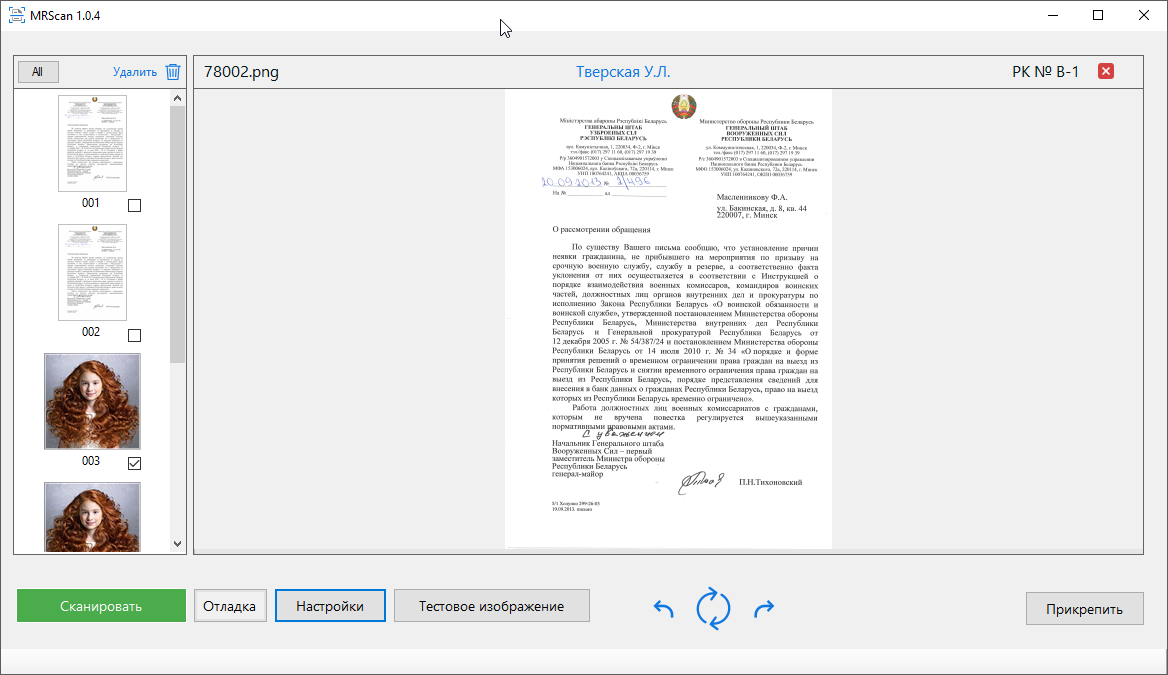
\includegraphics[scale=0.4]{mainSession.png}
	\caption{Главное окно с сессией}
	\clearpage
\end{figure}

Однако если десктопное приложение не установлено на компьютере, в браузере откроется всплывающее окно, уведомляющее об отсутствии приложения. Так же в окне будет ссылка по которой можно скачать инсталятор для MRScan (рисунок 7.5).

\begin{figure}[h!]
\centering
	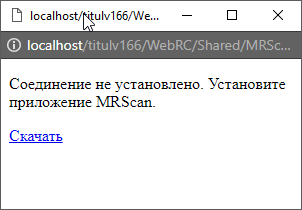
\includegraphics[scale=0.8]{mrsnotfound.png}
	\caption{Предупрежедение что приложение не установлено}
	\clearpage
\end{figure}

\subsubsection{Окно настроек}

На главном окне приложения расположена кнопка «Настройки». Если на нее нажать откроется новое окно с настройками приложения. В данном окне устанавливается способ сканирования, выбирается сканер, устанавливается тип итоговых документов и т.д. Конфигурирование процесса сканирование и работы приложения определяется в окне настроек (рисунок 7.6).

\begin{figure}[h!]
\centering
	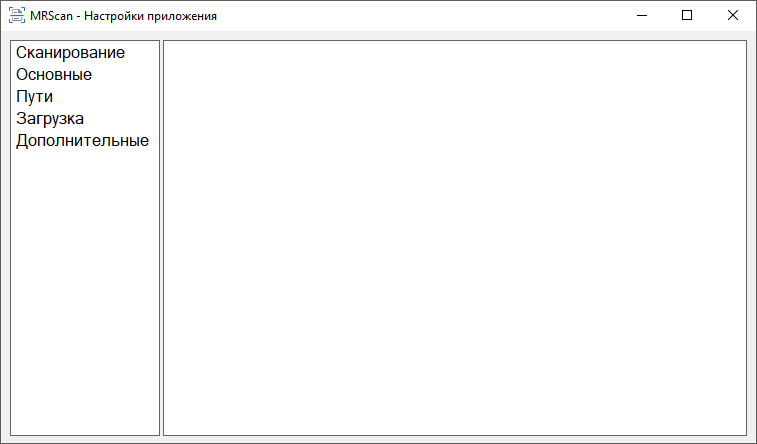
\includegraphics[scale=0.88]{generalsettings.png}
	\caption{Окно настроек}
	\clearpage
\end{figure}

Окно разделено на 5 вкладок.

Вкладка «Сканирование». На данной вкладке можно выбрать сканер и установить конфигурацию сканирования. Включить/Отключить двустороннее сканирование (рисунок 7.7)

\begin{figure}[h!]
\centering
	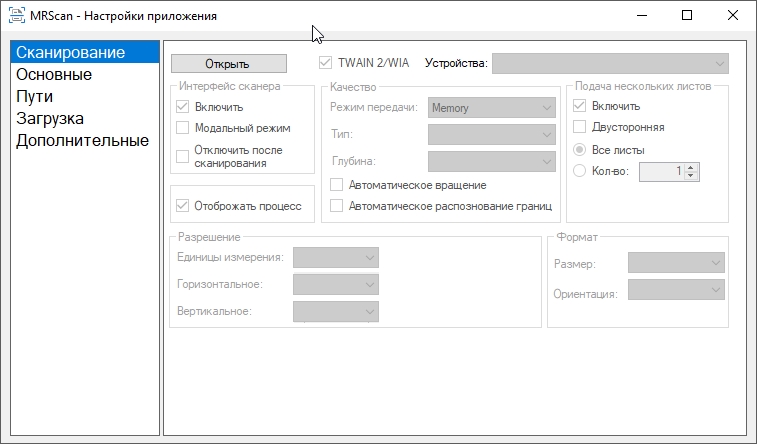
\includegraphics[scale=0.61]{tabScan.png}
	\caption{Вкладка «Сканирование»}
	\clearpage
\end{figure}

Вкладка «Загрузки»  (рисунок 7.8). На данной вкладке конфигурирется свойства прикрепляемых файлов. Для одностраничного типа файла, выбирается префикс, который будет добавлен для каждой странички. Для многостраничного типа файла есть чекбокс «Предлагать ввести имя файла», если он установлен, перед прикреплением документа, будет открываться окно, в которое пользователь должен ввести желаемое имя для файла. Если чекбокс неактивен, файлу будет дано униальное имя. 

\begin{figure}[h!]
\centering
	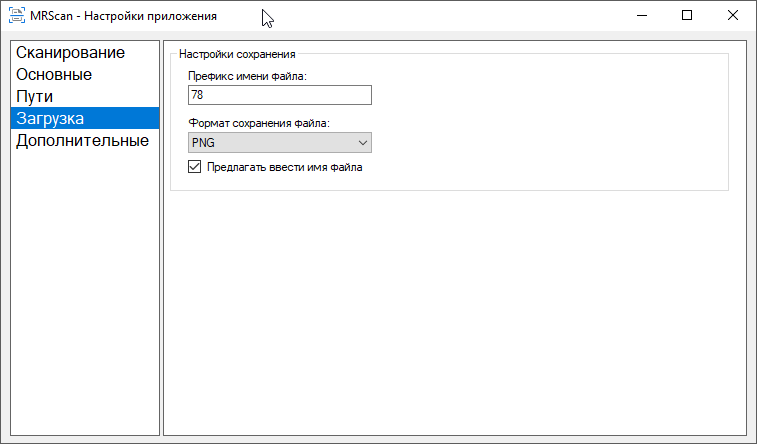
\includegraphics[scale=0.61]{tabDownload.png}
	\caption{Вкладка «Загрузка»}
	\clearpage
\end{figure}

Так же на этой вкладке из выпадающего списка выбирается формат сохранения фалов (рисунок 7.9).

\begin{figure}[h!]
\centering
	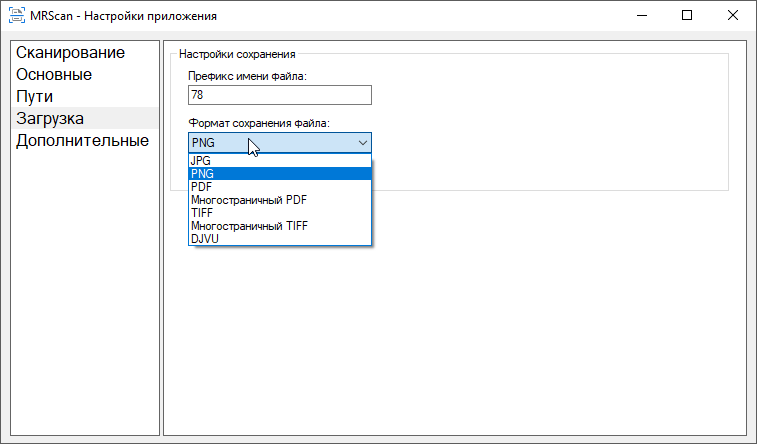
\includegraphics[scale=0.61]{tabDownloadList.png}
	\caption{Доступные форматы файлов}
	\clearpage
\end{figure}
